\documentclass[11 pt, handout]{beamer}
\let\Tiny=\tiny

\usepackage{mathtools}
\usepackage{amsfonts}
\usepackage{amsmath}
\usepackage{graphicx}
\usepackage{pgfpages}
\usepackage[]{xcolor}
\usepackage{tikz}


\newcommand{\meo}[1]{\texttt{#1}} % My Eyes Only: notes just for me
\newcommand{\bigo}{\mathcal{O}}
\newcommand{\extra}[1]{{\color{purple} {#1}}}

\usetheme{default}
\usecolortheme{beaver}
\usefonttheme{serif}


\beamertemplatenavigationsymbolsempty
\setbeameroption{show notes}


\newif\ifpresstime
	\presstimefalse
	% \presstimetrue

\mode<presentation>{
	\setbeameroption{hide notes}
}
\mode<handout>{
	\setbeameroption{show notes}
	\pgfpagesuselayout{2 on 1}[letterpaper, border shrink=5mm]

}


\ifpresstime
		\renewcommand{\meo}[1]{}
		\date{April 13, 2018}
		\setbeameroption{hide notes}
	\else
		\setbeameroption{show notes}
		% \setbeameroption{show only notes}
		\date{\today}
	\fi

\usetikzlibrary{arrows, automata, shapes}
\tikzset{
		initial text = {\scriptsize{\textsc{start}}},
		initial distance = 1 pt,
		every initial by arrow/.style={->},
		elliptic state/.style={draw,rounded rectangle},
		accepting/.style ={thick, double}
	}


\title{Kleene's Theorem}
\author{James McFeeters}
\institute {Beloit College}
\begin{document}

\frame{
	\titlepage
}

\begin{frame}
	\frametitle{Basic Definitions}
	\begin{itemize}
		\item Symbol
		\pause
		\item Alphabet ($\Sigma$)
		\pause
		\item String / word
		\begin{itemize}
			\pause
			\item The empty string ($\lambda$)
			\pause
			\item $|\lambda| = 0$
		\end{itemize}
		\pause
		\item Language
	\end{itemize}
\end{frame}


\begin{frame}
	\frametitle{Regular Operations}
	\begin{itemize}
		\item Union
		\item Concatenation
		\item Kleene Closure
	\end{itemize}
\end{frame}

\begin{frame}
	\frametitle{Concatenation}
	\begin{columns}[T]
		\column{0.3\textwidth}
			\begin{block}{Strings}
				\begin{flalign*}
					w_1 &= ab &\\
					w_2 &= bc &\\
					w_1 w_2 &= abbc &\\
				\end{flalign*}
			\end{block}
		\column{0.5\textwidth}
		\pause
			\begin{block}{Languages}
				\begin{flalign*}
					AB &= \{ ab \mid a \in A, \, b \in B \} &\\
				\end{flalign*}
			\end{block}
	\end{columns}
	\begin{columns}[T]
		\column{0.3\textwidth}
		\pause
			\begin{flalign*}
				w^0 &= \lambda 		& \\
				w^1 &= w 			& \\
				w^2 &= ww			& \\
				w^k &= w w^{k-1} 	&
			\end{flalign*}
		\column{0.5\textwidth}
		\pause
			\begin{flalign*}
				A^0 &= \{ \lambda\} 					& \\
				A^1 &= A \{ \lambda \} = A 				& \\
				A^2 &= AA = \{ xy \mid x, y \in A \}	& \\
				A^k &= A A^{k-1}
			\end{flalign*}
	\end{columns}
\end{frame}

\begin{frame}
	\frametitle{Kleene Closure}
	$A^*$: the \textit{Kleene closure} of $A$.
	\pause
	\begin{align*}
		A^* &= \bigcup_{k \geq 0} A^k \\
		&= \{ \lambda \} \cup A \cup A^2 \cdots \\
	\end{align*}
	\pause
	If $A = \{ y \}$ then $A^* = \{ \lambda, \: y, \: yy, \: yyy, \: \dots\}$.
\end{frame}





\begin{frame}
	\frametitle{Finite Automata}

	5-tuple: $M = (Q, \Sigma, s, \delta, F)$

	\begin{itemize}
		\pause
		\item $Q$ The set of possible states.
		\pause
		\item $\Sigma$ The alphabet of input symbols.
		\pause
		\item $s$ The initial state, $s \in Q$.
		\pause
		\item $\delta$ The transition function:
		\pause
		\[
			\delta: (Q \times \Sigma) \to Q.
		\]
		\pause
		\item $F$ The set of accepting states, $F \subseteq Q$.
	\end{itemize}
\end{frame}

\begin{frame}
	\frametitle{Regular Languages}

	The \textit{atomic} regular languages over an alphabet $\Sigma$ are
	\begin{itemize}
		\pause
		\item $\emptyset$
		\pause
		\item $\{ \lambda \}$
		\pause
		\item $\{ a \}$ for any $a \in \Sigma$ 
	\end{itemize}~\\[1 em]
	\pause

	If $A$ and $B$ are regular languages, then so are
	\begin{itemize}
		\pause
		\item $A \cup B$
		\pause
		\item $AB$
		\pause
		\item $A^*$
	\end{itemize}
\end{frame}



\begin{frame}
	\frametitle{Building a Finite Automaton}
	\centering
	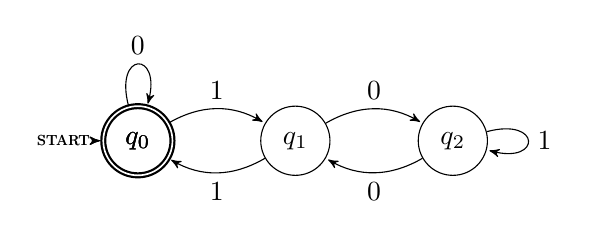
\begin{tikzpicture}[>=stealth',shorten >=1pt,auto,node distance=2cm]
		\pause
		\temporal<3>
		{\node[state] (q0)                 {$q_0$};}
		{\node[state, initial] (q0)                 {$q_0$};}
		{\node[state, initial, accepting] (q0)                 {$q_0$};}

		\node[state]                   (q1) [right of = q0] {$q_1$};
		\node[state]                   (q2) [right of = q1] {$q_2$};
		\pause
		\pause
		\pause
		\path[->] (q0) edge [loop above] node {0} (q0);
		\pause
		\path[->] (q0) edge [bend left]  node {1} (q1);
		\pause
		\path[->] (q1) edge [bend left]  node {0} (q2);
		\pause
		\path[->] (q1) edge [bend left]  node {1} (q0);
		\pause
		\path[->] (q2) edge [bend left]  node {0} (q1);
		\pause
		\path[->] (q2) edge [loop right] node {1} (q2);
	\end{tikzpicture}
\end{frame}





\begin{frame}[shrink]
	\frametitle{References}
	\bibliographystyle{amsplain}
	\nocite{*}
	\bibliography{../paper/references.bib}
\end{frame}

\end{document}
